\subsection{Euler equation for HD}
\begin{frame}{Introduction}
\begin{block}{Riemann problem in 2D}
	A Riemann problem consists of a system of conservation equation together with a piecewise constant initial condition.
\begin{tabular}{l l}
	\begin{minipage}{0.61\textwidth}
				\begin{equation*}
						U_t + F(U)_x + G(U)_y = 0
					\end{equation*}
					\begin{equation*}
						U_0(x,y) = 
						\begin{cases} u_1 & (x,y)  \in [0.5,1]^2 \\ 
						u_2 & (x,y)  \in [0,0.5]\times[0.5,1] \\ 
						u_3 & (x,y)  \in [0,0.5]^2 \\ 
						u_4 & (x,y)  \in [0.5,1]\times[0,0.5] \\ 
						\end{cases}
					\end{equation*}
	\end{minipage}
	&
	\begin{minipage}{0.4\textwidth}
	\hspace{10mm}
		\begin{figure}
			\centering
			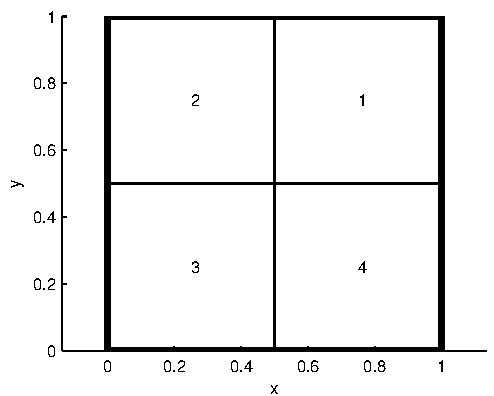
\includegraphics[width=\textwidth]{../src2/figs/init.pdf}
		\end{figure}
	\end{minipage}
	\end{tabular}
	\end{block}
\end{frame}

\begin{frame}{The equations}

\begin{block}{Euler equation for compressible fluids}
\begin{equation*}
U_t + F(U)_x + G(U)_y = 0
\end{equation*}
with
\begin{equation*}
U =
 \begin{pmatrix}
 \rho \\
 \rho u \\
 \rho v \\
 e
 \end{pmatrix} \hspace{5 mm}
 F =
  \begin{pmatrix}
  \rho u\\
  \rho u^2 + p \\
  \rho u v\\
  u(e+p)
  \end{pmatrix} \hspace{5 mm}
   G =
    \begin{pmatrix}
    \rho v\\
    \rho u v \\
    \rho u^2 + p \\
    v(e+p)
    \end{pmatrix} \hspace{5 mm}
\end{equation*}
Equation describing the dynamics of a compressible fluid.
Conserved quantities are: $ \rho $ density, $ \rho u $ momentum in $ x $ , $ \rho v$ momentum in $ y $ and the total energy $ e $.
\end{block}

\end{frame}



